%%% Thesis Introduction --------------------------------------------------
\chapter{Introduction}


\ifpdf
    \graphicspath{{Introduction/IntroductionFigs/PNG/}{Introduction/IntroductionFigs/PDF/}{Introduction/IntroductionFigs/}}
\else
  \graphicspath{{Introduction/IntroductionFigs/EPS/}{Introduction/IntroductionFigs/}}
\fi

\section{Overview}
\markboth{}{Node Failures and its Impact on Data Aggregation Delay}{}

This chapter can explain the introduction in general to your seminar work. then specifically you can have sub sections and sub-sub sections to explain each and every sub-area of your work. It can include a general introduction, advantages and challenges of the area.\\[1ex]

The rest of the report is organized as follows: A literature survey is presented in section 2. Two level Balanced and Progressive sensor network topologies and their energy optimization are described in section 3. In sections 4 to 6, we analyse node failure handling strategies in different levels of the Balanced and Progressive two level tree WSNs and propose solutions. Section 7 contains results and observations. Finally we conclude in section 8. \\[1ex]

\section{New Section}
%\markboth{}{\MakeUppercase{\thechapter.  Introduction }}
contents for section here....
\subsection{Subsection1}
You can write contents for your subsection here...

\subsection{Subsection2}

You can write contents for your subsection here...


\section{Another Section}
\markboth{}{Node Failures and its Impact on Data Aggregation Delay}{}

%\markboth{\MakeUppercase{\thechapter. Introduction }}

The enumeration:\\[1ex]
\begin{enumerate}
\item \textbf{Enum1}: Explanation1
\item \textbf{Enum2}: Explanation2
\end{enumerate}

The figure \ref{fig1} is \cite{RW1} : \\[1ex]

\begin{figure}[t]
\centering
\subfloat[Without In-Network Data Aggregation]{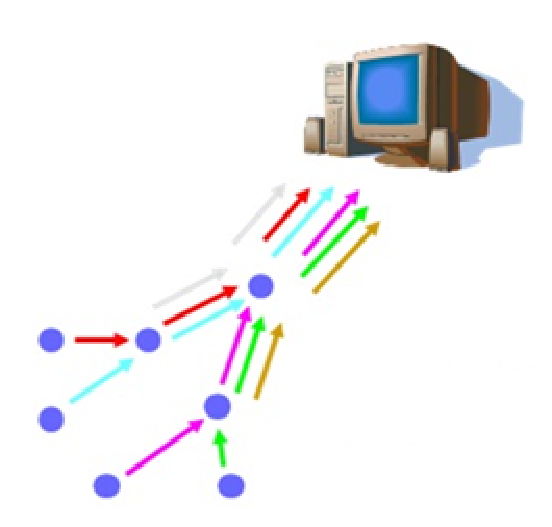
\includegraphics[width = 2.5in]{fig1.eps}}
\qquad
\subfloat[With In-Network Data Aggregation]{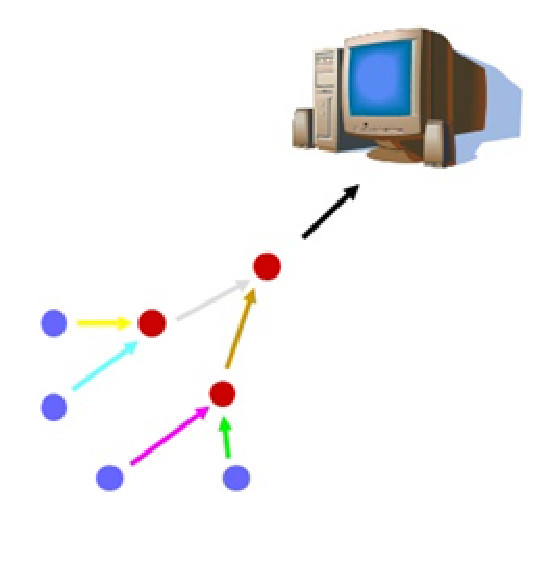
\includegraphics[width = 2.5in]{fig2.eps}}
\caption{In-Network Data Aggregation}
\label{fig1}
\end{figure}

Itemization: \\[1ex]
\begin{itemize}
\item Centralized Approach: This is an address centric approach where each node sends data to a central node via the shortest possible route using a multi hop wireless protocol.
\item In-Network Aggregation: In-network aggregation is the global process of gathering and routing information through a multi-hop network, processing data at intermediate nodes with the objective of reducing resource consumption (in particular energy), thereby increasing network lifetime. 
\item Tree-Based Approach: In the tree-based approach perform aggregation by constructing an aggregation tree, which could be a minimum spanning tree, rooted at sink and source nodes are considered as leaves.
\item Cluster-Based Approach: In cluster-based approach, whole network is divided in to several clusters. Each cluster has a cluster-head which is selected among cluster members \cite{RW2}.
\end{itemize}


%% Local Variables: 
%%% mode: latex
%%% TeX-master: "../thesis"
%%% End: 
